%  A simple AAU report template.
%  2015-05-08 v. 1.2.0
%  Copyright 2010-2015 by Jesper Kjær Nielsen <jkn@es.aau.dk>
%
%  This is free software: you can redistribute it and/or modify
%  it under the terms of the GNU General Public License as published by
%  the Free Software Foundation, either version 3 of the License, or
%  (at your option) any later version.
%
%  This is distributed in the hope that it will be useful,
%  but WITHOUT ANY WARRANTY; without even the implied warranty of
%  MERCHANTABILITY or FITNESS FOR A PARTICULAR PURPOSE.  See the
%  GNU General Public License for more details.
%
%  You can find the GNU General Public License at <http://www.gnu.org/licenses/>.
%
%!TEX root = ../master.tex

\documentclass[11pt,a4paper, openany]{report}

\usepackage[utf8]{inputenc}
% Make latex understand and use the typographic
% rules of the language used in the document.
\usepackage[french,english]{babel}
% Use the palatino font
\usepackage[sc]{mathpazo}
\linespread{1.05}         % Palatino needs more leading (space between lines)
% Choose the font encoding
\usepackage[T1]{fontenc}
%%%%%%%%%%%%%%%%%%%%%%%%%%%%%%%%%%%%%%%%%%%%%%%%
% Graphics and Tables
% http://en.wikibooks.org/wiki/LaTeX/Importing_Graphics
% http://en.wikibooks.org/wiki/LaTeX/Tables
% http://en.wikibooks.org/wiki/LaTeX/Colors
%%%%%%%%%%%%%%%%%%%%%%%%%%%%%%%%%%%%%%%%%%%%%%%%
% load a colour package
\usepackage{xcolor}
\definecolor{aaublue}{RGB}{33,26,82}% dark blue
% The standard graphics inclusion package
\usepackage{graphicx}
% Set up how figure and table captions are displayed
\usepackage{caption}
\captionsetup{%
  font=footnotesize,% set font size to footnotesize
  labelfont=bf % bold label (e.g., Figure 3.2) font
}
% Make the standard latex tables look so much better
\usepackage{array,booktabs}
% Enable the use of frames around, e.g., theorems
% The framed package is used in the example environment
\usepackage{framed}

%%%%%%%%%%%%%%%%%%%%%%%%%%%%%%%%%%%%%%%%%%%%%%%%
% Mathematics
% http://en.wikibooks.org/wiki/LaTeX/Mathematics
%%%%%%%%%%%%%%%%%%%%%%%%%%%%%%%%%%%%%%%%%%%%%%%%
% Defines new environments such as equation,
% align and split 
\usepackage{amsmath}
% Adds new math symbols
\usepackage{amssymb}
% Use theorems in your document
% The ntheorem package is also used for the example environment
% When using thmmarks, amsmath must be an option as well. Otherwise \eqref doesn't work anymore.
\usepackage[framed,amsmath,thmmarks]{ntheorem}

%%%%%%%%%%%%%%%%%%%%%%%%%%%%%%%%%%%%%%%%%%%%%%%%
% Page Layout
% http://en.wikibooks.org/wiki/LaTeX/Page_Layout
%%%%%%%%%%%%%%%%%%%%%%%%%%%%%%%%%%%%%%%%%%%%%%%%
% Change margins, papersize, etc of the document
\usepackage[
  inner=28mm,% left margin on an odd page
  outer=41mm,% right margin on an odd page
  ]{geometry}
% Modify how \chapter, \section, etc. look
% The titlesec package is very configureable
\usepackage{titlesec}
\titleformat{\chapter}[display]{\normalfont\huge\bfseries}{\chaptertitlename\ \thechapter}{20pt}{\Huge}
\titleformat*{\section}{\normalfont\Large\bfseries}
\titleformat*{\subsection}{\normalfont\large\bfseries}
\titleformat*{\subsubsection}{\normalfont\normalsize\bfseries}
% \titleformat*{\paragraph}{\normalfont\normalsize\bfseries}
% \titleformat*{\subparagraph}{\normalfont\normalsize\bfseries}

% Clear empty pages between chapters
\let\origdoublepage\cleardoublepage
\newcommand{\clearemptydoublepage}{%
  \clearpage
  {\pagestyle{empty}\origdoublepage}%
}
\let\cleardoublepage\clearemptydoublepage

% Change the headers and footers
\usepackage{fancyhdr}
\pagestyle{fancy}
\fancyhf{} %delete everything
\renewcommand{\headrulewidth}{0pt} %remove the horizontal line in the header
\fancyhead[R]{\small\nouppercase\leftmark} %even page - chapter title
\fancyheadoffset[R]{2cm}
\fancyhead[L]{\small\nouppercase\rightmark} %uneven page - section title
\fancyfoot[L]{\thepage} %page number on all pages
\fancyfoot[R]{Branch : \texttt{\branch}} %git branch
% Do not stretch the content of a page. Instead,
% insert white space at the bottom of the page
\raggedbottom
% Enable arithmetics with length. Useful when
% typesetting the layout.
\usepackage{calc}

%%%%%%%%%%%%%%%%%%%%%%%%%%%%%%%%%%%%%%%%%%%%%%%%
% Bibliography
% http://en.wikibooks.org/wiki/LaTeX/Bibliography_Management
%%%%%%%%%%%%%%%%%%%%%%%%%%%%%%%%%%%%%%%%%%%%%%%%
\usepackage[backend=bibtex,
  bibencoding=utf8
  ]{biblatex}
\addbibresource{bib/mybib}
\usepackage{csquotes}

%%%%%%%%%%%%%%%%%%%%%%%%%%%%%%%%%%%%%%%%%%%%%%%%
% Misc
%%%%%%%%%%%%%%%%%%%%%%%%%%%%%%%%%%%%%%%%%%%%%%%%
% Add bibliography and index to the table of
% contents
\usepackage[nottoc]{tocbibind}
% Add the command \pageref{LastPage} which refers to the
% page number of the last page
\usepackage{lastpage}
% Add todo notes in the margin of the document
\usepackage[
%  disable, %turn off todonotes
  colorinlistoftodos, %enable a coloured square in the list of todos
  textwidth=\marginparwidth, %set the width of the todonotes
  textsize=scriptsize, %size of the text in the todonotes
  ]{todonotes}

%%%%%%%%%%%%%%%%%%%%%%%%%%%%%%%%%%%%%%%%%%%%%%%%
% Hyperlinks
% http://en.wikibooks.org/wiki/LaTeX/Hyperlinks
%%%%%%%%%%%%%%%%%%%%%%%%%%%%%%%%%%%%%%%%%%%%%%%%
% Enable hyperlinks and insert info into the pdf
% file. Hypperref should be loaded as one of the 
% last packages
\usepackage{hyperref}
\hypersetup{%
	% pdfpagelabels=true,%
	plainpages=false,%
	pdfauthor={Author(s)},%
	pdftitle={Title},%
	pdfsubject={Subject},%
	bookmarksnumbered=true,%
	colorlinks=false,%
	citecolor=black,%
	filecolor=black,%
	linkcolor=black,% you should probably change this to black before printing
	urlcolor=black,%
	pdfstartview=FitH%
}

\usepackage{ifxetex}
\usepackage{textpos}
\usepackage{kpfonts}
\usepackage{stackengine}

%% Adition by Froux 
\usepackage{listings} % Required for insertion of code
\usepackage[boxed]{algorithm2e}
\usepackage{courier} % Required for the courier font
\usepackage{lipsum} % Used for inserting dummy 'Lorem ipsum' text into the template
\usepackage{tikz} % Used for drawing figures and graphs

\usepackage{ntheorem}
\theoremstyle{break}
\newtheorem{lemma}{Lemma}
\newtheorem{theorem}{Theorem}
\newtheorem{remark}{Remark}
\newtheorem{definition}{Definition}
\newtheorem{proof}{Proof}% package inclusion and set up of the document
%!TEX root = ../master.tex
%%%%% Notation provided in the imperial College Template %%%%%

% quick way of adding a figure
\newcommand{\fig}[3]{
 \begin{center}
 \scalebox{#3}{\includegraphics[#2]{#1}}
 \end{center}
}

\newcommand{\figcap}[4]{
 \begin{figure}[ht]
        \centering
        \scalebox{#4}{\includegraphics[#2]{#1}}
        \caption{#3}
    \end{figure}
}

%\newcommand*{\point}[1]{\vec{\mkern0mu#1}}
\newcommand{\ci}[0]{\perp\!\!\!\!\!\perp} % conditional independence
\newcommand{\point}[1]{{#1}} % points 
\renewcommand{\vec}[1]{{\boldsymbol{{#1}}}} % vector
\newcommand{\mat}[1]{{\boldsymbol{{#1}}}} % matrix
\newcommand{\R}[0]{\mathds{R}} % real numbers
\newcommand{\Z}[0]{\mathds{Z}} % integers
\newcommand{\N}[0]{\mathds{N}} % natural numbers
\newcommand{\nat}[0]{\mathds{N}} % natural numbers
\newcommand{\Q}[0]{\mathds{Q}} % rational numbers
\ifxetex
\newcommand{\C}[0]{\mathds{C}} % complex numbers
\else
\newcommand{\C}[0]{\mathds{C}} % complex numbers
\fi
\newcommand{\tr}[0]{\text{tr}} % trace
\renewcommand{\d}[0]{\mathrm{d}} % total derivative
\newcommand{\inv}{^{-1}} % inverse
\newcommand{\id}{\mathrm{id}} % identity mapping
\renewcommand{\dim}{\mathrm{dim}} % dimension
\newcommand{\rank}[0]{\mathrm{rk}} % rank
\newcommand{\determ}[1]{\mathrm{det}(#1)} % determinant
\newcommand{\scp}[2]{\langle #1 , #2 \rangle}
\newcommand{\kernel}[0]{\mathrm{ker}} % kernel/nullspace
\newcommand{\img}[0]{\mathrm{Im}} % image
\newcommand{\idx}[1]{{(#1)}}
\DeclareMathOperator*{\diag}{diag}
\newcommand{\E}{\mathds{E}} % expectation
\newcommand{\var}{\mathds{V}} % variance
\newcommand{\gauss}[2]{\mathcal{N}\big(#1,\,#2\big)} % gaussian distribution N(.,.)
\newcommand{\gaussx}[3]{\mathcal{N}\big(#1\,|\,#2,\,#3\big)} % gaussian distribution N(.|.,.)
\newcommand{\gaussBig}[2]{\mathcal{N}\left(#1,\,#2\right)} % see above, but with brackets that adjust to the height of the arguments
\newcommand{\gaussxBig}[3]{\mathcal{N}\left(#1\,|\,#2,\,#3\right)} % see above, but with brackets that adjust to the height of the arguments
\DeclareMathOperator{\cov}{Cov} % covariance (matrix) 
\ifxetex
\renewcommand{\T}[0]{^\top} % transpose
\else
\newcommand{\T}[0]{^\top}
\fi
% matrix determinant
\newcommand{\matdet}[1]{
\left|
\begin{matrix}
#1
\end{matrix}
\right|
}


%%% various color definitions
\definecolor{darkgreen}{rgb}{0,0.6,0}

\newcommand{\blue}[1]{{\color{blue}#1}}
\newcommand{\red}[1]{{\color{red}#1}}
\newcommand{\green}[1]{{\color{darkgreen}#1}}
\newcommand{\orange}[1]{{\color{orange}#1}}
\newcommand{\magenta}[1]{{\color{magenta}#1}}
\newcommand{\cyan}[1]{{\color{cyan}#1}}


% redefine emph
\renewcommand{\emph}[1]{\blue{\bf{#1}}}

% place a colored box around a character
\gdef\colchar#1#2{%
  \tikz[baseline]{%
  \node[anchor=base,inner sep=2pt,outer sep=0pt,fill = #2!20] {#1};
    }%
}%


%%%%% Adition by Froux %%%%%


\newcommand{\abs}[1]{\mid#1\mid} % Valeur Absolue
\newcommand{\norm}[1]{ \mid \mid #1\mid \mid } %Norme d'un vecteur


%----------------------------------------------------------------------------------------
%	CODE INCLUSION CONFIGURATION
%----------------------------------------------------------------------------------------

\definecolor{MyDarkGreen}{rgb}{0.0,0.4,0.0} % This is the color used for comments
\lstloadlanguages{C} % Load Perl syntax for listings, for a list of other languages supported see: ftp://ftp.tex.ac.uk/tex-archive/macros/latex/contrib/listings/listings.pdf
\lstset{language=python, % Use python in this example
        frame=single, % Single frame around code
        basicstyle=\small\ttfamily, % Use small true type font
        keywordstyle=[1]\color{Blue}\bf, % Perl functions bold and blue
        keywordstyle=[2]\color{Purple}, % Per function arguments purple
        keywordstyle=[3]\color{Blue}\underbar, % Custom functions underlined and blue
        identifierstyle=, % Nothing special about identifiers                                         
        commentstyle=\usefont{T1}{pcr}{m}{sl}\color{MyDarkGreen}\small, % Comments small dark green courier font
        stringstyle=\color{Purple}, % Strings are purple
        showstringspaces=false, % Don't put marks in string spaces
        tabsize=5, % 5 spaces per tab
        %
        % Put standard Perl functions not included in the default language here
        morekeywords={rand},
        %
        % Put Perl function parameters here
        morekeywords=[2]{on, off, interp},
        %
        % Put user defined functions here
        morekeywords=[3]{test},
       	%
        morecomment=[l][\color{Blue}]{...}, % Line continuation (...) like blue comment
        numbers=left, % Line numbers on left
        firstnumber=1, % Line numbers start with line 1
        numberstyle=\tiny\color{Blue}, % Line numbers are blue and small
        stepnumber=5 % Line numbers go in steps of 5
}

% Creates a new command to include a perl script, the first parameter is the filename of the script (without .pl), the second parameter is the caption
\newcommand{\script}[2]{
\begin{itemize}
\item[]\lstinputlisting[caption=#2,label=#1]{#1.c}
\end{itemize}
}


%% This insert part of a PDF -> This is an exemple for a 2 slides per page pdf.
\newcommand{\slide}[1]{
\begin{center}

\ifodd#1
\includegraphics[page= \numexpr (#1/2), clip, scale=0.7, viewport=110 460 500 780]{Cours1}
\else
\includegraphics[page=\numexpr (#1/2), clip, scale=0.7, viewport=110 100 500 380]{Cours1}
\fi
\end{center}
}



\newcommand{\aautitlepage}[2]{%
  {
    %set up various length
    \ifx\titlepageleftcolumnwidth\undefined
      \newlength{\titlepageleftcolumnwidth}
      \newlength{\titlepagerightcolumnwidth}
    \fi
    \setlength{\titlepageleftcolumnwidth}{0.5\textwidth-\tabcolsep}
    \setlength{\titlepagerightcolumnwidth}{\textwidth-2\tabcolsep-\titlepageleftcolumnwidth}
    %create title page
    \thispagestyle{empty}
    \noindent%
    \begin{tabular}{@{}ll@{}}
      \parbox{\titlepageleftcolumnwidth}{
        
\includegraphics[width=\titlepageleftcolumnwidth]{figures/imperial}
       } &
      \bigskip\\
       #1 &
      \parbox[t]{\titlepagerightcolumnwidth}{%
      \textbf{Abstract:}\bigskip\par
        \fbox{\parbox{\titlepagerightcolumnwidth-2\fboxsep-2\fboxrule}{%
          #2
        }}
      }\\
    \end{tabular}
    \vfill
    
      \noindent{\footnotesize\emph{The content of this report is freely available, but publication (with reference) may only be pursued due to agreement with the author.}}
    
    \clearpage
  }
}

%Create english project info
\newcommand{\englishprojectinfo}[4]{%
  \parbox[t]{\titlepageleftcolumnwidth}{
    \textbf{Title:}\\ #1\bigskip\par
    \textbf{Theme:}\\ #2\bigskip\par
    \textbf{Period:}\\ #3\bigskip\par
    \textbf{Page Numbers:} \pageref{LastPage}\bigskip\par
    \textbf{Date of last change:}\\ #4
  }
}

%%%%%%%%%%%%%%%%%%%%%%%%%%%%%%%%%%%%%%%%%%%%%%%%
% An example environment
%%%%%%%%%%%%%%%%%%%%%%%%%%%%%%%%%%%%%%%%%%%%%%%%
\theoremheaderfont{\normalfont\bfseries}
\theorembodyfont{\normalfont}
\theoremstyle{break}
\def\theoremframecommand{{\color{gray!50}\vrule width 5pt \hspace{5pt}}}
\newshadedtheorem{exa}{Example}[chapter]
\newenvironment{example}[1]{%
        \begin{exa}[#1]
}{%
        \end{exa}
}% my new macros

\begin{document}
%frontmatter
\pagestyle{empty} %disable headers and footers
\pagenumbering{roman} %use roman page numbering in the frontmatter
%!TEX root = ../master.tex
%  A simple AAU report template.
%  2015-05-08 v. 1.2.0
%  Copyright 2010-2015 by Jesper Kjær Nielsen <jkn@es.aau.dk>
%
%  This is free software: you can redistribute it and/or modify
%  it under the terms of the GNU General Public License as published by
%  the Free Software Foundation, either version 3 of the License, or
%  (at your option) any later version.
%
%  This is distributed in the hope that it will be useful,
%  but WITHOUT ANY WARRANTY; without even the implied warranty of
%  MERCHANTABILITY or FITNESS FOR A PARTICULAR PURPOSE.  See the
%  GNU General Public License for more details.
%
%  You can find the GNU General Public License at <http://www.gnu.org/licenses/>.
%
\pdfbookmark[0]{Front page}{label:frontpage}%
\begin{titlepage}
  \addtolength{\hoffset}{0.5\evensidemargin-0.5\oddsidemargin} %set equal margins on the frontpage - remove this line if you want default margins
  \noindent%
  \begin{tabular}{@{}p{\textwidth}@{}}
    \toprule[2pt]
    \midrule
    \vspace{0.2cm}
    \begin{center}
    \Huge{\textbf{
      Machine Learning and AI % insert your title here
    }}
    \end{center}
    \begin{center}
      \Large{
        - Methods and Algorithms  -% insert your subtitle here
      }
    \end{center}
    \vspace{0.2cm}\\
    \midrule
    \toprule[2pt]
  \end{tabular}
  \vspace{4 cm}
  \begin{center}
    {\large
      Personnal Notes %Insert document type (e.g., Project Report)
    }\\
    \vspace{0.2cm}
    {\Large
      François Bouvier d'Yvoire%Insert your group name or real names here
    }
  \end{center}
  \vfill
  \begin{center}
  CentraleSupélec \& Imperial College \\
  Current Branch : \texttt{\branch} \\
  Commit : \texttt{\commit} 
  \end{center}
\end{titlepage}
\clearpage
\pdfbookmark[0]{Contents}{label:contents}
\pagestyle{fancy} %enable headers and footers again
\tableofcontents
\listoftodos
%mainmatter

% 
%!TEX root = ../master.tex
\chapter*{Intro} % (fold)
\label{cha:intro}

This document will use the following classification for the machine learning algorithms. However their might be some changes. For exemple, some of them will be part of the commons algorithms and not from their real class. 

\begin{figure}[ht]
\centering
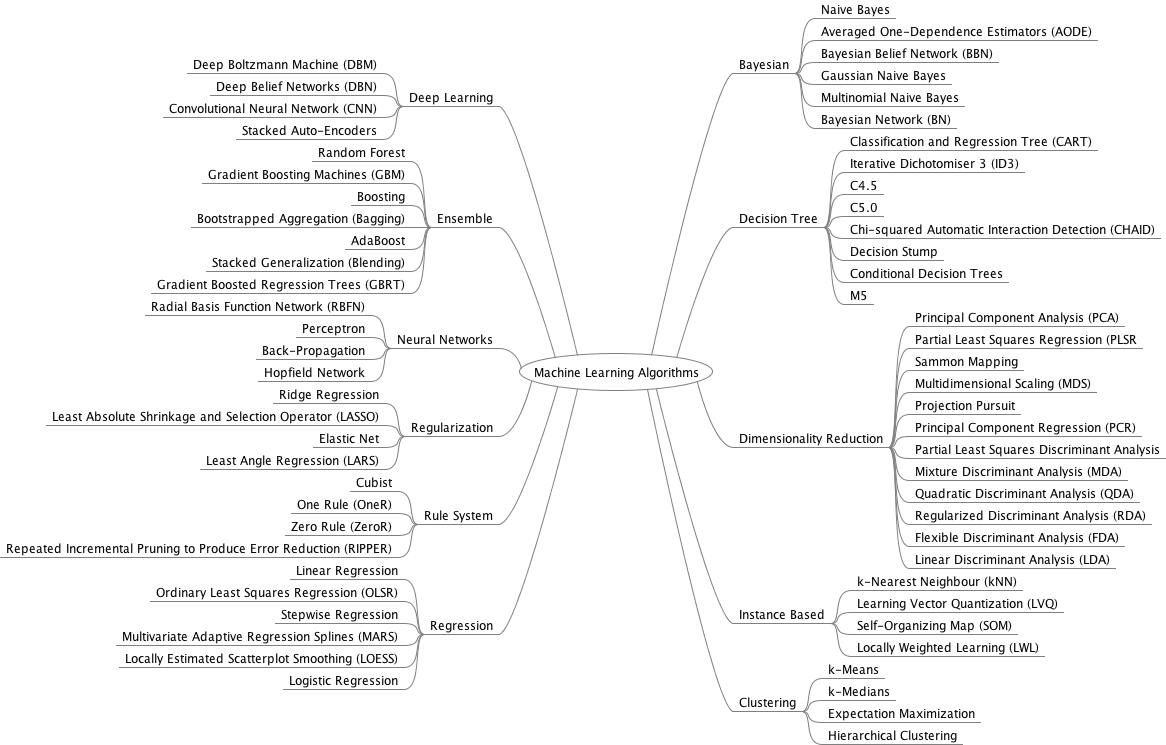
\includegraphics[scale=0.4]{figures/MachineLearningAlgorithms}
\caption{Simple graph for algorithms classification in ML}
\end{figure}

% chapter intro (end)
\pagenumbering{arabic} %use arabic page numbering in the mainmatter
%!TEX root = ../master.tex
\chapter{Logic-Based Learning} % (fold)
\label{cha: logic_learning}


	\section{Inductive Logic Programming (ILP)} % (fold)
	\label{sec:inductive_logic_programming}
		
		\subsection{Introduction to Concept Learning}

			In Concept Learning we aim to compute a definition of a concept, expressed in a given langage (called \emph{hypothesis space}) that satisfies positive exemple and none of negatives ones. As an exemple, it can be a regexp which can match all words of a set, and none of an other set (see Regexp Golf) 
	% section inductive_logic_programming (end)
% chapter  (end logic_learning)
%!TEX root = ../master.tex
\chapter{Common Machine Learning algorithms}\label{ch:introduction}

This chapter is dedicated to the most common ML algorithms, a major part of the notes come from the mml-books.com \todo{Add bibtex reference}

It is intended to introduce different concept used in most Machine Learning Algorithms before moving to more specific algorithms.

\section{What is Machine Learning ?}

\todo{Add short intro that explain the goal, the process, etc of Machine Learning}
\section{Graphical Model for Probabilistic Inference}

Based on the Probabilistic Inference Course of Marc Deisenroth (Imperial College)

	\subsection{Probabilistic Pipeline}

	Here is a simple pipeline of the inference process with a model

		\figcap{figures/pipeline_proba}{}{Simple Pipeline of how to build model for inference}{0.8}

	\subsection{Probabilistic graphical Model}

		In order to deal with complex and big probalistic model, we can use different kind of graphs which represent relationships between random variables. We define the random variables as nodes and the probabiistic or functional relationship between variables as edges in the graphs. With them you can :
		\begin{itemize}
			\item Visualize the structure
			\item Have insights into properties (such as conditional independance)
			\item Design or Motivate new models
			\item Compute some inference and learning as graphical manipulations
		\end{itemize}

		There exists 3 kinds of model : Bayesian networks (directed graphical models), Markov random fields (undirected graphical models) and factor graphs (with nodes which are not random variables)/

		\subsubsection{Bayesian Networks}

			\todo[inline]{add basic graphs exemple}

			They are defined by 
			\begin{itemize}
				\item Nodes : Random variables
				\item Shaded nodes: Observed random variables
				\item Other : Latent Variables
				\item Edges : (a, b) $\iff$ conditionnal distribution $p(b|a)$
			\end{itemize}

			\todo[inline]{add graphicals model of linear regression}

			\paragraph*{D-Separation:} A set A of nodes is d-Separated (conditionnaly independant) from B by C iff all path between A and B are blocked. C is tht set of observed variables in the graphical model.
			\begin{definition}
				A Path is \emph{Blocked} id it includes a node such that either :
				\begin{itemize}
					\item The arrow on the path meet either head-to-tail or tail-to-tail at the node, and the node is in C 
					\item The arrow meet head-to-head at the node, and neither the node nor any of its descendants is in the set C
				\end{itemize}
			\end{definition}

			\paragraph*{Markov Random Fields}
				Defined by : if X and Y are not connected directly, then X and Y are conditionnaly independant given everything else.

				Then Joint distributions are the product of cliques in the graphs, and the full joint (of all variables) is the product of the joint of the maximum cliques

				\[
					p(x) = fra{1}{Z} \Pi _C \psi _C(x_C)
				\]
				Where C describe a maximal clique, $x_C$ all the variable in C, $\psi_C$ the clique potential and Z a normalisation constant. 

				Check for the condiational independance : Check if when remmoving the observable variable there is no path between two set of random variable.

				The potentials can be seen as Energy Functions, which mean we can write $\psi_C(x_C) = exp(-E(x_C))$ with E some energy functions, and then $-log(p(x)) = \sum_C E(x_C)$ is the sum of energies of the clique potential.


				\todo[inline]{Add Image Denoising exemple}

			\paragraph*{Factor Graphs}

				(Un)directed graphical models express a global function of several variables as a product of factors over subsets of those variables

				Factor graphs make this decomposition explicit by introducing additional nodes for the factors themselves


\section{Linear Regression}

	The Linear regression problem correspond to find a linear mapping $f(x)$ based on noisy observation $y = f(x) + \epsilon$, where $\epsilon$ is a noise. 
	Finding the regression function require : 
	\begin{itemize}
		\item Choice of parameters (function classes, dimension)
		\item Choice of probabilistic model (Loss function, ...)
		\item Avoiding under and overfitting
		\item Modeling uncertainty on data
	\end{itemize}

	\begin{definition}
			\begin{itemize}
				\item $p(x, y)$ is te joint distribution
				\item $p(x)$ and $p(y)$ are the marginal distributions
				\item $p(y|x)$ is the conditional distribution of $y$ given $x$
			 	\item in the context of regression, $p(y|x)$ is called likelihood, $p(x|y)$ the posterior, $p(x)$ the prior and $p(y)$ the marginal likelihood or evidence.
			 	\item they are related by the Bayes' Theorem : $p(x|y) = \frac{p(y|x)p(x)}{p(y)}$ 
			\end{itemize}
		\end{definition}

	\subsection{Conjugacy} % (fold)
	\label{sub:conjugacy}
		In order to compute the posterior, we require some calculations which imply the prior, and can be intractable as a closed form. But given a likelihood, it can exist prior which give closed-form solution for the posterior. This is the principle of conjugacy (between the likelihood and the prior)
	% subsection conjugacy (end)

	\subsection{Maximum Likelihood Estimation (MLE)}
	In order to obtain the parameters, we need to choose a quantity to optimize. The first and most common idea is to choose the Likelihood as a cost function to optimize. The seems natural because the likelihood represent the probability given the $X$ variables to obtain the observed variables $Y$ and we want this to be maximum on the known data (which are the training set).

	\[
		\theta^* = \arg \max_{\theta} p(y | X, \theta)
	\]

	To find the desired parameters that maximize the likelihood, we typically do gradient ascent (or gradient descent on the negative likelihood). For numerical reasons, we apply the log-transformation to the probleme and minimize the negative log-likelihood. 

		\paragraph*{Closed-Form Solution - Linear Regression}

			In some cases, a closed-form solution exist, which make computation easy (but not necesseraly cheap)

		\paragraph*{MLE with Features}

	\subsection{Overfitting}

	\subsection{Regularization}
	\subsection{Maximum A Posteriori Estimation (MAP)}

		\paragraph*{MAP for Linear Regression}

\section{Gradient Descent}

	\subsection{Simple Gradient Descent}

	\subsection{Gradient Descent with Momentum}

	\subsection{Stochastic Gradient Descent}


\section{Model Selection and Validation}

	\subsection{Cross-Validation}

	\subsection{Bayesian Model Selection}
		\paragraph*{Bayes Factor}

		\paragraph*{Fully Basyesian Treatment}

	\subsection{Marginal Likelihood}

\section{Bayesian Linear Regression}

	\subsection{Mean and Variance}

	\subsection{Sample function}

\section{Features Extraction}
	\todo{Simply explain and redirect to relevant chapter (dim reduc, computer vision, ...)}

\section{Support Vector Machine}

	\subsection{Linear Separating Hyperplane}

		\paragraph*{Lagrangian duality}
		\paragraph*{Karush-Kuhn-Tucker Condition for Optimality}
	\subsection{SVM dual problem}

	\subsection{Support Vector Regression}






%!TEX root = ../master.tex
\chapter{Bayesian Algorithms} % (fold)
\label{cha:bayesian_algorithms}

	Bayesian Algorithms aims to produce not just function (for classification or regression) but distribution over function, which achieve to get the uncertainty of our model according to the uncertainty of the data.

	\section{Gaussian Process}

		This section is made with a great inspiration from the Probabilistic Inference from Marc Deisenroth (Imperial College London)
		\subsection{Problem setting} % (fold)
		\label{sub:problem_setting}
			For a set of observation $y_i = f(x_i) + \epsilon$ with $\epsilon \sim \mathcal{N}(0, \sigma_\epsilon^2$, we want to fine a distribution over \emph{functions} $p(f)$ that explains the data. It's not exactly the same as a linear regression problem because we do not look for only one function.

			This is a really power full process used in a lot of different problematic thanks to its robustness and known properties (in comparison to deep learning methods).

			\begin{itemize}
				\item Reinforcement Learning and Robotics
				\item Bayesian optimization
				\item Geo-statistics 
				\item Sensor networks
				\item Time-series modelling and forecasting
				\item High-energy physics
				\item Medical application
			\end{itemize}

			Formally a Gaussian Process is a multivariate Gaussian distribution with infinite variables (countable or even uncountable).

		% subsection problem_setting (end)
		\subsection{Definition} % (fold)
		\label{sub:definition}
			A Gaussian process is defined by a mean function $m(\dot)$ and a covariance function (=kernel) $k(\dot, \dot)$.

			The mean function represents the average of all the function.\\
			the Covariance function allows us to compute covariance between any two functions. Notes that the function are unknown, and only this correlations are fully known.
			% subsection definition (end)

		\subsection{Gaussian Process Inference} % (fold)
		\label{sub:gaussian_process_inference}
				
			Considering $X$ training inputs and $y$ training target, the Bayes' theorem in the case of Gaussian Process become 
			\[
				p(f | X, y) = \frac{p(y | f, X)p(f)}{p(y | X)}
			\]
			Which gives us a Likelihood $p(y | f, X) = \mathcal{N}(f(X), \sigma^2 \mat I)$, a Marginal Likelihood $p(y | X) = \int p(y | f, X) p (f | X) df$ and a Posterior $p(f |y, X) = \textbf{GP}(m_{post}, k_{post})$

			How can we manage to work with the distribution over function, and then infinite dimension for calculus, etc. ? This is possible because each time you consider only finite sample, computing the joint distribution boils down to work on finite-dimensional multivariate Gaussian distributions

			Then we can use the gaussian properties (including gaussian prior as conjugate, ...) to make prediction : \\
			(We define $X_*, f_*$, etc as the test data and predicted function)
			\[
				p(f(x_*) | X, y, x_*) = \mathcal{N}(m_{post}(x_*), k_{post}(x_*, x_*))
			\]

			This can also be seen as 
			\[
				p(f(x_*) | X, y, x_*) = \mathcal{N}(\text{E}{[f_* | X, y, X_*]}, V{[f_* | X, y, X_*]})
			\]
			with $\text{E}[f_* | X, y, X_*] =$ prior mean + "Kalman gain" * error $= m(X_*) + k(X_*, X)(\mat K + \sigma^2_n \mat I)^{-1}(y-m(X))$ and $V [f_* | X, y, X_*] = k(X_*, X_*) - k(X_*, X)(\mat K + \sigma^2_n \mat I)^{-1})k(X, X_*)$

			% subsection gaussian_process_inference (end)

		\section{Bayesian Optimisation}
% chapter bayesian_algorithms (end)
%!TEX root = ../master.tex
\chapter{Deep Learning} % (fold)
\label{cha:deep_learning}

\section{Intro}
	\subsection{Representation Learning}

		Representation Learning is the field where you try to learn the representation (features) of input. Then you can do classification or regression on the representative space.

	\subsection{Deep Learning vrsus classical Representation Learning}
		\todo[inline]{Add image with where Deep Learning is relative to ML}


\section{Optimisation : Gradient Descent}
	\subsection{Stochastic GD versus Mini-Batch}

		Classicaly the learning is an optimization problem : 
		\[
			\hat \theta = \arg \min_\theta \frac{1}{n}\sum^n_1 l(f_\theta(x_i), y_i)
		\]

		Then we can calculate a gradient
		\[
			\nabla_\theta \hat L (\theta) = \frac{1}{n}	\sum^n_1 \nabla_\theta l(f_\theta(x_i), y_i)
		\]

		There is different possibility to update the parameters, the stochastic way (SGD) which learn only one by one exemple:

		\[
			\theta^{(t+1)} = \theta^{(t)} - \alpha^{(t)} \nabla_\theta l(f_\theta(x_{t}), y_{t})
		\]

		And the mini-batch which average the learning on a mini-batch (b < n the data set size) of examples.
		\[
			\theta^{(t+1)} = \theta^{(t)} - \alpha^{(t)} \frac{1}{b}\sum^b_1 \nabla_\theta l(f_\theta(x_{tb+i}), y_{tb+i})
		\]

	\subsection{Convergence rate and computational complexity}
		
		\[
			\mathbb{E}(\hat L(\theta^{(k)} - \hat L(\theta^*))) \leq \frac{\alpha \sigma^2}{2m}+ (1 -\alpha m )^k (\hat L(\theta^{(0)} - \hat L(\theta^*)))
		\]

		With conclusion : 
		\begin{itemize}
		 	\item Small step size $\implies$ \emph{Slower} initial convergence and Stalls at \emph{more} accurate result
			\item Large step size $\implies$ \emph{Faster} initial convergence and Stalls at \emph{less} accurate result
			\item Small batch size $\implies$ Stalls at \emph{less} accurate result and \emph{Lower} iteration cost
			\item  Small batch size $\implies$ Stalls at \emph{more} accurate result and \emph{Higher} iteration cost
		\end{itemize}

	\subsection{Deep Learning is not convex}
			which mean you don't know if local extrema is global extrema, and this is problematic for gradient descent method, which find local extrema.

			\todo[inline]{Add ref to convexity}


\section{Maximum Likelihood estimation}

	\todo[inline]{Kullback-Leibler divergence}
	\todo[inline]{cross entropy}
	\todo[inline]{Log-likelihood}
	\todo[inline]{$L_2$ as MLE} 
	\todo[inline]{Logistic Regression}

\section{Regularization}

	In order to avoid certain problem (overfiting, saturation...) regularization can be added to the loss function, (can be named weight decay). This works in restricting the hypothesis class, and find explanation in different way, such as Ockahm Razor. 

	\subsection{Generality}
		General form : 
		\[
			\min_\theta \hat L(\theta) + \beta R(\theta)
		\]
		\begin{itemize}
			\item Soft constraint
			\item Equivalent to hard constraint (Lagrangian)
			\item equivalent to the Maximum a posteriori interpretation (see Common ML)
		\end{itemize}

		The regularization reduce the capacity of the model, so a trade-off exist between large capacity but under-regularisation (overfitting or not convergence) and small capacity with over-regularization

		\paragraph*{Bayesian view}
			todo{fill MAP equation}

	\subsection{Geometric interpretation}

	\subsection{$L_1$ Regularization}

	\subsection{Noisy input}
		We can show that add an i.i.d noise $\epsilon \sim \mathit{N}(0, \beta \mat I)$ is equivalent to weight decay.
	\subsection{Data Augmentation}

	\subsection{Early stopping}

	\subsubsection*{Dropout}

	\subsection{Covariate shift}

	\subsection{Batch normalization}

	\subsection{Input pre-processing}
		\begin{itemize}
			\item Zero-centered data
			\item normalized data
			\item Decorrelated data
			\item Whitened data
		\end{itemize}
\section{Deep Feed-forward network}
	\subsection{Perceptron}
		\paragraph*{Activation function}
			\begin{itemize}
				\item tanh
				\item sigmoid
				\item ReLU -> Logistic regression
		\end{itemize}

		\paragraph*{Multi-layer perceptron}
			Single layer is not enough
			\todo[inline]{XOR Problem}
			\begin{theorem}
				A perceptron with one hidden layer of finite width can arbitrarily accurately approximate any continuous function on a compact
				subset of $\mathbb{R}^n$ (under mild assumptions on the activation function)
			\end{theorem}

		\paragraph*{What is better: Depth or Width ?}

		\paragraph*{Popular output layer types}
			\begin{itemize}
				\item 1D Regression
				\item Binary classification
				\item nD Regression
				\item Softmax (multi-class classification)
			\end{itemize}

		\paragraph*{Backpropagation}
			Use chain rule to calculate all the layer gradient relative to the output gradient.
			\todo[inline]{Differentiable programming}


\section{Deep convolutionnal Neural network}

	See Imaging chapter first


% chapter deep_learning (end)
%!TEX root = ../master.tex
\chapter{Ensemble Algorithms} % (fold)
\label{cha:ensemble_algorithms}


Idea : Aggregate the predictions of a group of predictors (either classifiers or regressors)

In many case the aggregated answer is better than best individual prediction. \todo[inline, color=green]{add illustration from ML for imaging course}

Even weak learner can achieve high accuracy, provided there are un sufficient number and sufficently diverse. 

\todo[inline, color=green]{Voting toy exemple ?}

\begin{definition}
	\begin{itemize}
		\item Homogenous Ensemble Learning
		Use the same class of ML model (which are Weak Learner)
		\item Heterogenous Ensemble Learning
		Use different ML model
		\item  Sequential : Base Learners are added one at a time, mislabelled
examples are upweighted each time(Ex : Boosting)
		\item Parallel : many independent base learners are trained
simultaneously and then combined (Ex : Voting, Bagging, Random Forest)
	\end{itemize}
\end{definition}

\begin{definition}
	\emph{Weak Learner} :  is defined to be a classifier that is only slightly
correlated with the true classification (0.5 for bi-classifier)
\end{definition}


\section{Bagging : Boostrap Aggregating}

	Reduce model variance through averaging
	\todo[inline]{Add Bootstrapping 3 steps and Aggregating}

	\subsection{Outof-bag error}

\section{Boosting}

	\subsection{Principle}
	Rather than building independent weak learners in parallel and
aggregating at end:
– build weak learners in serial
– but adaptively reweight training data prior to training each new weak learner
– in order to give a higher weight to previously misclassified examples

	\subsection{Exemple ?}

\subsection{Several variants}
• Adaboost (adaptive boosting)
– Originally for classification
– Can be used for regression too
• Gradient Tree Boosting
• XGBoost

\subsubsection*{Adaboost}
	Adaboost = Adaptive Boosting


	\todo[inline]{Optimizing Adaboost with early termination}

\section{Decision Trees}


% chapter ensemble_algorithms (end)
%!TEX root = ../master.tex
\chapter{Imaging} % (fold)
\label{cha:imaging}

\section{Image Classification}

	\subsection{Features and Classifier}

	\subsection{Feature Extraction - without ML}

	\begin{itemize}
	 	\item Why features ?
	 	\item What features should be : \\
	 		– Distinctive and discriminative
			– Local (to enable establishing correspondences)
			– Invariant to viewpoint changes or transformations (translations/rotations)
			– Invariant to illumination changes
			– Efficient to compute
			– Robust to noise and blurring
			– Should be hierarchical

		\item Many options possible : – Intensities
									– Gradient
									– Histogram
									– SIFT
									– SURF
									– BRIEF
		\item Pixel level bad : Not discriminative, Localiser and does not represent local pattern, not invariant to transformation. 
		\item Patch Level : More discriminative, Not necessarily rotation invariant, semi-localised. Use Convolution for patch. 
		\item Image Level : discriminative, Not localised, not necessarily rotation invariant. Get a feature map where each pixel correspond to local pattern
	 \end{itemize} 

	 How to make rotation invariant ? $ \rightarrow $ Use Histogram.
	 \subsubsection{Filtering}

		- Use filter to identify features such as gradient, edge detection.\\
		- Gradient are invariant to absolute illumination.

	\subsubsection{SIFT}

	\begin{itemize}
		\item Scale-space Extrema Detection : For all scale, compute convolution with gaussian (blur at different level) and compute the difference of each scaled guassian, then Detect local extrema of Differences
		\item Keypoint Localisation : 
		\item Orientation Assignment : Take a small window around the keypoint location.An orientation histogram with 36 bins
		covering 360 degrees is created.
		Each pixel votes for an orientation bin,
		weighted by the gradient magnitude
		after applying a Gaussian filter with
		he keypoint scale !).
		The keypoint will be assigned an
		orientation, which is the mode of the
		distribution
		\item Keypont descriptors.
	\end{itemize}

	\subsubsection{OHoG (Histogram of Gradient)} % (fold)
	\label{sub:hog_}
	
	% subsection hog (end)
	
	\subsubsection{SURF (Speeded-Up Robust Features)} % (fold)
	\label{sub:surf}
	
	% subsection surf (end)

	\subsubsection{BRIEF (Binary Robust Independant Elementary Features)} % (fold)
	\label{sub:brief_}
	
	% subsection brief_ (end)

	\subsubsection{Local binary Patterns} % (fold)
	\label{sub:local_binary_patterns}
	
	% subsection local_binary_patterns (end)

	\subsubsection{Haar features} % (fold)
	\label{sub:haar_features}
	
	Convolution ineficient $\rightarrow$ Faster computation via integral images S
	% subsection haar_features (end)
	
	\subsection{with ML} % (fold)
	\label{sub:with_ml}
	
		\todo{Add Classical ML pipeline for computer vision (images, features, classification)}

		Classification or regression model, many options : Logistic regression, Naives Bayes, K-Nearest neighbors, Support vector Machines (does not deal good with computer vision \todo{why ?}, Boosting, Decision/Random forsest, Neural network.

		Boosting and Decision trees are Ensemble forests. 
	% subsection with_ml (end)

	\todo[inline]{add bias-variance error explanation in common ML}

% chapter imaging (end)
% %!TEX root = ../master.tex

\chapter{Reinforcement Learning} % (fold)
	\label{cha:reinforcement_learning}


\section{Markov Reward and Decision Process} % (fold)
	\label{sec:markov_reward_and_decision_process}

	\subsection{State Value Function Closed-form} % (fold)
		\label{sub:state_value_function}
		
		For a Markov Reward Process ($\mathcal{S}, \mathcal{P}, \mathcal{R}, \gamma$), defining the Return $\mathsf R_t$ and the State Value Function
		$\mathsf v (s) = \mathbb{E}[\mathsf R_t  S_t = s]$\\
		Then we have, in a vector form : 
		\[
			\mathbf{v} = (\mathbb{1} - \gamma \mathcal P )^{-1} \mathcal{R}
		\]
		Unfortunately, Matrix inversion in costly, so this is only feasible in small Markov Reward Process
	% subsection state_value_function (end)

	\subsection{Iterative Policy Evaluation Algorithm} % (fold)
		\label{sub:iterative_policy_evaluation_algorithm}

	% subsection iterative_policy_evaluation_algorithm (end)
% section markov_reward_and_decision_process (end)

\section{Dynamic Programming in RL} % (fold)
	\label{sec:dynamic_programming_in_rl}

	\subsection{Policy Iteration Algorithm} % (fold)
		\label{sub:policy_iteration_algorithm}
		
	% subsection value_iteration_algorithm (end)

	\subsection{Value Iteration Algorithm} % (fold)
		\label{sub:value_iteration_algorithm}
	
	% subsection policy_iteration_algorithm (end)

	\subsection{Assynchronous Backup in RL} % (fold)
		\label{sub:assynchronous_backup_in_rl}
		
		\paragraph{Prioritised Sweeping} % (fold)
			\label{par:prioritised_sweeping}
		
		% paragraph prioritised_sweeping (end)

		\paragraph{Real-time Dynamic Programming} % (fold)
			\label{par:real_time_dynamic_programming}
		
		% paragraph real_time_dynamic_programming (end)

	% subsection assynchronous_backup_in_rl (end)
	
	\subsection{Properties and drawbacks of Dynamic Programming} % (fold)
		\label{sub:properties_and_drawbacks_of_dynamic_programming}
	
	% subsection properties_and_drawbacks_of_dynamic_programming (end)

% section dynamic_programming_in_rl (end)

\section{Model-Free Learning} % (fold)
	\label{sec:model_free_learning}

	\subsection{Monte-Carlo Algorithms} % (fold)
		\label{sub:monte_carlo_algorithm}

		\paragraph*{(First Visit) Monte-Carlo Policy Evaluation}

		\paragraph*{Every Visit Monte-Carlo Policy Evaluation}

		\todo{Add "you cannot backup death" explanations}

		\paragraph*{Batch vs Online Monte-Carlo}

		\paragraph*{Incremental Monte-Carlo Update}

		\paragraph*{Runing Mean for Non-Stationnary World}
	% subsection monte_carlo_algorithms (end)

	\subsection{Monte-Carlo Control Algorithms} % (fold)
		\label{sub:monte_carlo_control_algorithms}
	
		\paragraph*{Monte-Carlo Policy Improvement}

			\subparagraph*{Greedy Policy Improvement over State Value Function}

			\subparagraph*{Greed Policy Improvement over State-Action Value Function}

		\paragraph*{Exploring Starts Problem}
			\todo{Don't forget Starting to explore}

		\paragraph*{On Policy Soft Control}
		
		\paragraph*{On-Policy $\epsilon$-greedy first-visit Monte-Carlo control Algorithm}

		\paragraph*{Monte-Carlo Batch Learning to Control}

		\paragraph*{Monte-Carlo Iterative Learning to Control}
	% subsection monte_carlo_control_algorithms (end)

	\subsection{Temporal Difference Learning} % (fold)
		\label{sub:temporal_difference_learning}
		
		\paragraph*{Temporal Difference Value Function Estimation Algorithm}
	% subsection temporal_difference_learning (end)
	\todo{Add Comparison between MC and TD learning}

	\subsection{Temporal Difference Learning Control Algorithm} % (fold)
		\label{sub:temporal_difference_learning_control_algorithm}
		
		\paragraph*{SARSA - On Policy learning Temporal Difference Control}

			\subparagraph*{SARSA-Lambda}
			\subparagraph*{Hindsight Experience Replay}

		\paragraph*{Q-Learning: Off-Policy Temporal Difference Learning}

	% subsection temporal_difference_learning_control_algorithm (end)

% section model_free_learning (end)

\section{Reinforcement Learning with Function Approximation} % (fold)
	\label{sec:reinforcement_learning_with_function_approximation}

	\subsection{Exemple of features} % (fold)
		\label{sub:exemple_of_features}

		\paragraph*{Coarse Coding}
		\paragraph*{Tile Coding}
		\paragraph*{Radial-Basis Function}
		\paragraph*{Deep Learning}
	% subsection exemple_of_features (end)

	\subsection{Monte-Carlo with Value Function Approximation} % (fold)
		\label{sub:monte_carlo_with_value_function_approximation}
	
	% subsection monte_carlo_with_value_function_approximation (end)
	
	\subsection{Temporal Difference Learning with Value Function Approximation} % (fold)
	\label{sub:temporal_difference_learning_with_value_function_approximation}

	% subsection temporal_difference_learning_with_value_function_approximation (end)
	
	\subsection{Q-Learning with FA} % (fold)
	\label{sub:q_learning_with_fa}
	
	% subsection q_learning_with_fa (end)
	
	\subsection{subsection name} % (fold)
	\label{sub:subsection_name}
	
	% subsection subsection_name (end)
% section reinforcement_learning_with_function_approximation (end)

\section{Deep Learning Reinforcement Learning} % (fold)
	\label{sec:deep_learning_reinforcement_learning}

	\subsection{Experience Replay} % (fold)
		\label{sub:experience_replay}
	
	% subsection experience_replay (end)
	\subsection{Target Network} % (fold)
		\label{sub:target_network}
	
	% subsection target_network (end)
	\subsection{Clipping of Rewards} % (fold)
		\label{sub:clipping_of_rewards}
	
	% subsection clipping_of_rewards (end)
	\subsection{Skipping of Frames} % (fold)
	\label{sub:skipping_of_frames}
	
	% subsection skipping_of_frames (end)
% section deep_learning_reinforcement_learning (end)
% chapter reinforcement_learning (end)
% %!TEX root = ../master.tex
\chapter{Dimensionality Reduction} % (fold)
\label{cha:dimensionality_reduction}

\section{Principal Component Analysis} % (fold)
	\label{sec:principal_component_analysis}
	
	\subsection{Simple algorithm} % (fold)
		\label{sub:simple_algorithm}
	
	% subsection simple_algorithm (end)

	\subsection{Whitening PCA} % (fold)
		\label{sub:whitening_pca}
	
	% subsection whitening_pca (end)

	\subsection{Kernel PCA} % (fold)
		\label{sub:kernel_pca}
	
	% subsection kernel_pca (end)
% section principal_component_analysis (end)
	
% chapter dimensionality_reduction (end)

% %!TEX root = ../master.tex
\chapter{Argumentation Framework} % (fold)
\label{cha:argumentation_framework}

This chapter are notes from the Imperial Course Machine Arguing from Francesca Toni. \todo{add ref}

\paragraph{introduction} % (fold)
\label{par:introduction}

	Argument Framework are a field in AI which provide way of evaluate any debate problem. It is useful to resolve conflict, to explain decision or to deal with incomplete information. 
% paragraph introduction (end)
\section{Abstract Argumentation}

	\subsection{Simple AA}

		\begin{definition}
		 		an  \textbf{AA framework} is a set $\mathrm{Args}$ of arguments and a binary relation $\mathrm{attacks}$. $(\alpha, \beta)\in \mathrm{attacks}$ means $\alpha$ attacks $\beta$.
		\end{definition} 

		\paragraph{Semantics in AA} 
			In order to define a "winning" set of argument, we need to provide semantics over the the framework. This is like recipes which determine good set of arguments. 

		\begin{definition}
			\begin{itemize}
				\item \textbf{conflict-free}
				\item \textbf{admissible:} c-f and attacks each attacking argument.
				\item \textbf{preferred:} maximally admissible.
				\item \textbf{complete:} admissible + contains each argument it defends.
				\item \textbf{stable:} c-f + attacks each argument not in it.
				\item \textbf{grounded:} minimally complete.
				\item \textbf{sceptically preferred:} Intersection of all prefered.
				\item \textbf{ideal:} maximal admissible and containing all prefered.
			\end{itemize}
		\end{definition}

		\begin{definition}
			\textbf{Semi-stable extension:} complete such as $A\cup A^+$ is maximal. $A^+$ is the set of attacked argument by $A$.
		\end{definition}

		\todo{add ref to ASPARTIX and CONARG}

	\subsection{Algorithms for AA}

		\paragraph{Computing the grounded labelling:}
		Here is an algorithm to compute a grounded labelling\\
		\begin{algorithm}[H]
		\KwData{An AA Framework}
		\KwResult{The grounded Labelling}
		Label all unatacked argument with IN \;
		\While{The IN and the OUT are not stable}
		{
			Label OUT the arguments attacks by IN \;
			Label IN the arguments only attacked by OUT\;
		}
		Label the still unlabelled UNDEC\;
		\caption{Computing the grounded labelling}
		\end{algorithm}

		\paragraph{Computing membership in preferred/grounded/ideal extensions;} In order to compute membership, we use Dispute Tree.

		We compute a dispute tree for an argument, and apply the different semantics which are easier to compute on a tree than on a graph.
		\todo{add algos of computing dispute tree + def of semantics}

		\paragraph{Computing stable extension:} We use answer set programming with logical program. 
		

	\subsection{AA with Suppport}

		\subsubsection[BAA]{Bipolar Abstract Argumentation}
			We add a \textbf{Support} relation to a classic AA Framework. There are different semantics, but we focus here one the QuAD (\textbf{Quantitative Argument Debate}) which add a numerical strenght to any argument, and give rule for updating strenght regarding the supporters or attackers.

			\todo{Add DF-QuAD rules and algorithm}
	\subsection{Argument Mining}
	\subsection{AA with Preference Probabilist}

\section{Assumption-Based Argumentation}

	\subsection{Simple ABA}
	\subsection{ABA more DDs}
	\subsection{p-acyclic ABA}

\section{ArgGame}
% chapter argumentation_framework (end)
% %!TEX root = ../master.tex

\chapter{Useful Computation} % (fold)
\label{cha:useful_computation}

\section{Data Centering using Matrix Multiplication} % (fold)
\label{sub:data_centering_using_matrix_multiplication}

\[
	\mat X- \mat M = \mat X\left( \mat I_n - \frac{1}{n} \mat 1_n \mat 1_n \T  \right)
\]

% subsection data_centering_using_matrix_multiplication (end)
% chapter useful_computation (end)
% \printbibliography[heading=bibintoc]
% \label{bib:mybiblio}

\end{document}